\chapter{Model, view and controller}
In this chapter we first give an overview of our implementation of Model-view-controller with its call dependencies. After the overview is a more detailed explanation of first the model, then the view and in the end the controller.  

In Figure \vref{fig:overview} is an overview how our model-view controller framework/architecture has been implemented in our application where the arrows is a call dependency. It is an incomplete representation for the program because not all Classes have been represented in the figure, however, all the connections between the controller and model has been represented. 

In the figure the Model's seven classes, sql\_helper excluded, are all used by at least one controller while the sql\_helper is used by the other classes to relay SQL commands to the database. The model will be further explained in section VREF{???????????}. We have implemented five views which corresponds to user interfaces for the Login and the contact book, the viewer will be explained further in section VREF{???????}. Four controllers has been implemented which function will be explain in section VREF{???????????}.

\begin{figure}[ht]
	\centering
		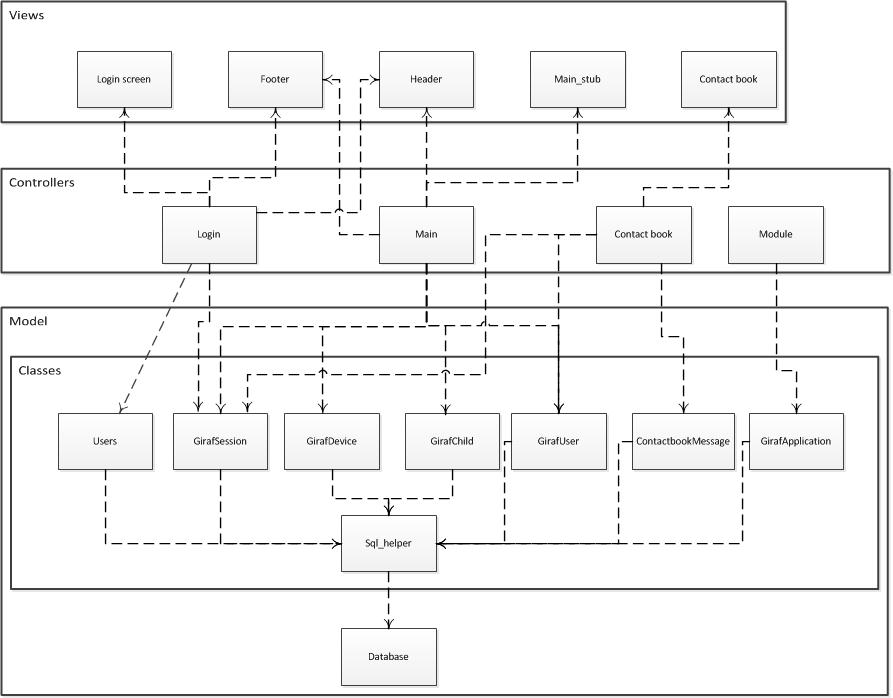
\includegraphics[width=0.80\textwidth]{img/overview.jpg}
	\caption{model-view-controller overview}
	\label{fig:overview}
\end{figure}
